% Chapter 4

% variables
\newcommand{\pdirfour}{chapters/plots/chapter4}

\chapter{Results} % Main chapter title

\label{chapter4} % For referencing the chapter elsewhere, use \ref{Chapter1}

In this chapter, we summarize the results of the NA64 experiment to this date, which include all the runs up to 2018, and are reported in detail in \cite{Banerjee:2020fue,Banerjee:2019hmi,NA64:2019imj,na64-prd,Banerjee:2018vgk,Banerjee:2016tad}. In the previous chapter, we did all the heavy lifting of estimating the background, calculating the systematic uncertainty, defining the selection criteria, and computing the signal yield. Now all is left to do is to un-blind the signal region and apply our selection criteria to the full sample, and simply count the number of events in the signal region that we defined. As the reader might already have guessed given no noble price has yet been awarded, no events were ever found in the signal region to this date. This leaves us with the task of deciding how to exactly cast our results in a useful way so that we are aware of what models are no longer a viable explanation to explain our cosmological measurements. This is done using the modified frequentist approach to compute the confidence level, taking the profile likelihood as test statistic in the asymptotic approximation \cite{Read_2002,JUNK1999435,Cowan:2010js}. This technique is summarized in Appendix.\ref{AppendixE}, and uses a representative data set provided by the Monte Carlo (also called Asimov data set) to obtain the median experimental sensitivity and its uncertainty.

To properly compare our results with all other experiments in the field, we chose the criteria of an 90\%C.L. as the upper limit, and we exclude the hypothesis $\dmhypo$ accordingly. The standard way to show this result is a plot in the $dmplane$ showing the region were all hypotheses are excluded, combined with relevant results of other experiments and interesting region for a physicist to explore. The most relevant example in our case of the relevant region is the one that explains the $\DMX$-anomaly as protophobic vector-boson \cite{PhysRevD.95.035017}. However, such a way of presenting the results completely ignores other parameters that are interesting for the cosmological models. Indeed, since we always performed our experiment under the assumption that a decay channel dominates and the $\DM$ itself is not interacting, the exact mass of the LDM $m_{\chi}$ and the dark sector coupling $\alpha_D$ do not change the results of our experiment. Therefore, the results are presented using the standard variable:

\begin{equation}
  \label{eq:y-dm}
  y = \epsilon^2 \alpha_D (m_{\chi}/m_{\DM})^4
\end{equation}

This variable takes into account all relevant parameters for our model and scales with the cross-section for the freeze-out.

%----------------------------------------------------------------------------------------

\section{Exclusion limits}
\label{ch4:sec:exclusion limits}

To date, no event has been recorded in the signal region defined for the invisible/visible mode setup. The results are shown in Fig.\ref{fig:exclusion-dmplane} that illustrates the models $\dmhypo$ excluded currently by the NA64 experiment. The plots were obtained by a detailed MC simulation of $\DM$ using different values of its parameter and applying all selection criteria. These simulations were then interpolated using a smooth Bézier interpolation of the points. An interesting feature that is immediately visible is the different shapes the exclusion region takes in the two plots. In the case of the invisible mode, the production of $\DM$ is sufficient for the experiment to detect it\footnote{Providing the event can pass all selection criteria, whose efficiency depends only weakly on the precise $\dmhypo$.}, so only the cross-section is limiting our signal yield. Looking at Eq.\ref{eq:dm-rate} back in Chapter 1, we see that the rate depends quadratically on both parameters of the theory. After accounting for some corrections of the selection criteria with the MC simulation, we produce as expected a curve similar to a parabola in the log-log plane, with large mass and low coupling harder to probe due to their low rate. Such reasoning does not help us with the visible mode parameter space, there is a part of the parameter space that is not yet covered even though the coupling $\epsilon$ is high and the mass relatively small. The reason as explored in Sec.\ref{ch3:sec:vis-mode-tracking} has to do with the efficiency of detection. Indeed such large coupling is bound to produce a very high number of $\DMM$, but we can see in Eq.\ref{eq:dm-decay-length} that the decay length is reducing at the same rate. Since we can only detect decays that happen outside the target, we need to consider the exponential distribution of the decay only from the end of the dump. We can convince ourselves that this means that the number of events will be exponentially suppressed because of this effect, and increasing the number of events contributes therefore only logarithmically to the signal yield. The result is what is seen in the plot, the exclusion region posses two regimes, one at $\epsilon < 10^{-4}$ dominated by the production of $\DMM$ that scales linearly with the EOTs accumulated and one at $\epsilon > 3 \times 10^{-4}$ dominated by the efficiency in detection that scales only logarithmically with them.

The $\DMX$ parameter space to date is excluded up to $\epsilon \simeq 6.8 \times 10^{-4}$ with the data collected in 2018. We saw in chapter \ref{chapter1} that to justify the $\DMX$-anomaly a coupling up to $\epsilon \simeq 1.4 \times 10^{-3}$ is allowed, which leaves us a particularly difficult region of the parameter space left to explore. It was my final task in this thesis to contribute to the design of an experiment able to cover the region in a feasible amount of time. This new design is covered in Sec.\ref{ch5:sec:new-vismode-setup}. One has also to be careful to interpret the experimental bound shown in the plot. For example, it appears from the plot that the NA48 experiment already covers a relevant region for $\DMX$ but this not true! Because of its (alleged) protophobic nature, the $\DMX$ cannot be searched in $\pi^0 \rightarrow \gamma \DM$ decay, this means those limit are only valid for the standard vector boson explored in Sec.\ref{ch1:sec:dm-u1model}, and it is not straight forward to extend it to more complex models. Also, we already saw that models that explain the $\DMX$-anomaly can vary a lot and have many different caveats, the plot here shows just the case of protophobic vector boson as described by Feng in \cite{Feng:2016jff}, but many other possibilities exist as well \cite{PhysRevD.95.035017}.

In the case of invisible mode, the main interest of the scientific community was if the $\DM$ can be a viable explanation for the anomalous magnetic moment of the muon $a_{\mu}$. At present, the data collected by NA64 rejects the hypothesis that the deviation of $a_{\mu}$ can be attributed to the $\DM$. This was confirmed independently by the BABAR experiment, which was the first one to publish a paper excluding completely this region of the parameter space \cite{PhysRevLett.119.131804}.

Finally, one more case under consideration was the one of ALPS\footnote{Axion Like Particles} and light scalar particles that couples to photons via the Primakoff effect. For this search, data from the invisible mode setup are used and the signal box is changed slightly: now only the first HCAL module is used as VETO, and the second and third modules are allowed to contain all the energy missing from the ECAL, as the ALPS (or light scalar) particle will decay $a(s) \to \gamma \gamma$ similarly to the visible mode. This search presents background slightly different from the one of the invisible mode, which was studied in \cite{Banerjee:2020fue}. The results are presented in Fig.\ref{}

\begin{figure}[tbh!]
  \centering
  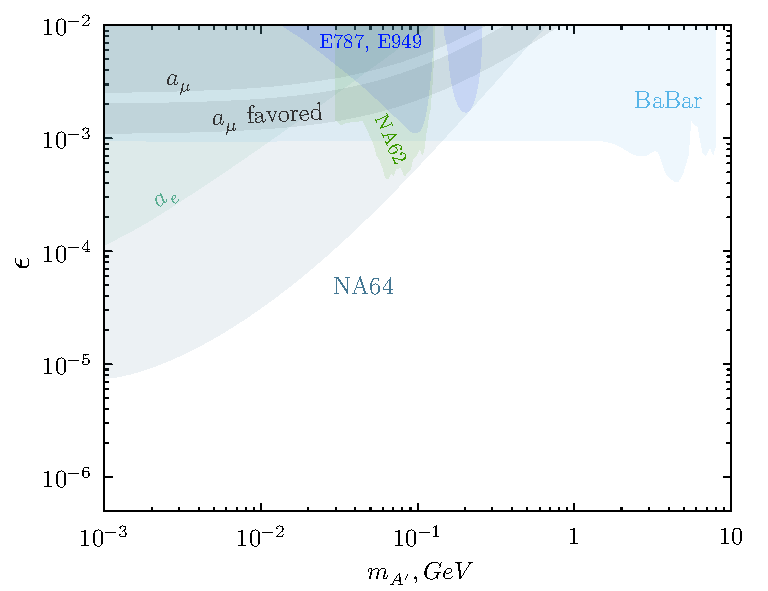
\includegraphics[width=0.45\textwidth,height=0.5\textwidth]{\pdirfour/exclusionInvisible.pdf}
  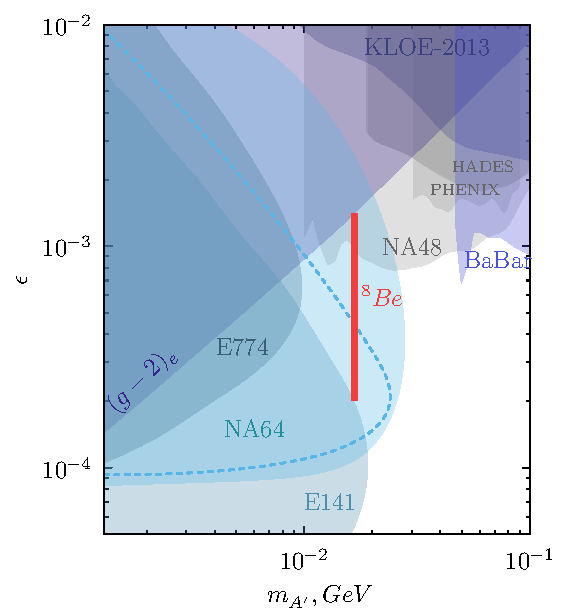
\includegraphics[width=0.45\textwidth,height=0.5\textwidth]{\pdirfour/exclusionVisible.pdf}
  \caption[Exclusion limits in the $\dmplane$]{The NA64 90\% exclusion region in the $\dmplane$ plane. The exclusion is shown for the data collected in the invisible mode setup (right) and visible mode setup (left), assuming the dominant decay is either invisible or visible respectively\cite{NA64:2019imj,Banerjee:2019hmi}. For the invisible mode, constraints from E787 and E949 \cite{PhysRevD.89.095006,Essig:2013vha},BABAR \cite{PhysRevLett.119.131804}, and recent NA62 results \cite{CortinaGil:2019nuo} are also shown, together with the muon $a_{\mu}$ favored area. For the visible mode, constraints from the experiments E774 \cite{PhysRevLett.67.2942}, E141 \cite{PhysRevLett.59.755}, BABAR \cite{babar1}, KLOE \cite{kloe2}, HADES \cite{hades}, PHENIX \cite{phenix}, NA48 \cite{na48} and bounds from the anomalous magnetic moment of the electron \cite{PhysRevD.89.095006} are shown. A blue dotted line shows the previous limit obtained with the analysis of the 2017 data. A thick red line shows the full parameter space that can justify the $\DMX$-anomaly \cite{PhysRevD.95.035017}, $2 \times 10^{4} < \epsilon< 1.4 \times 10^{-3}$. Currently, NA64 exclude coupling $\epsilon < 6.8 \times 10^{-4}$ for a $\DMX$ mass of 16.7 \mev.}
  \label{fig:exclusion-dmplane}
\end{figure}

\begin{figure}[bth!]
  \centering
  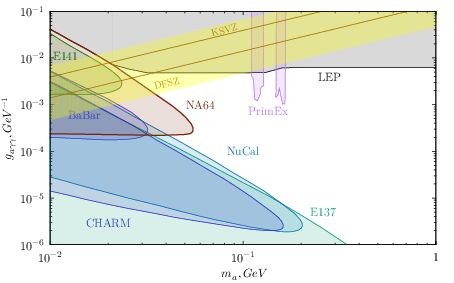
\includegraphics[scale=0.8]{\pdirfour/alps_new.png}
  \caption[Exclusion limits in the $(m_{a};g_{a \gamma \gamma})$ plane for ALPS and light scalar]{The 90\% exclusion limit for ALPS and light scalar particle obtained from the full dataset 2016-2018 in NA64 plotted in the $(m_{a};g_{a \gamma \gamma})$ plane. The yellow band represents the parameter space for the benchmark DFSZ \cite{DINE1981199} and KVSZ \cite{PhysRevLett.43.103} models. Constraint from BABAR \cite{Dolan:2017osp}, E137 \cite{e137}, E141 \cite{e141}, LEP , and PrimEx \cite{PhysRevLett.123.071801} experiments, as well as limits from CHARM \cite{BERGSMA1985458} and NuCal \cite{Dobrich:2019dxc} are also shown.}
  \label{fig:exclusion-dmplane-alps}
\end{figure}

While we are waiting for new results to shed some light on the $\DMX$-anomaly, we can study the impact of our results in the broader framework of cosmological dark matter. As detailed in chapter \ref{chapter1}, various dark sector models motivate sub-\gev scalar and Majorana or pseudo-Dirac fermium Dark Matter coupled to dark photons \cite{battaglieri2017cosmic}. We can use the requirement of the thermal freeze out of DM annihilation into visible matter to derive a relation between the interesting parameters of the model \cite{na64-prd}:

\begin{equation}
  \label{eq:ad-freeze-out}
  \alpha_D \simeq 0.02 f\left(\frac{10^-3}{\epsilon}\right)^2\left(\frac{m_{\DM}}{100 \mev}\right)^2\left(\frac{10 \mev}{m_{\chi}}\right)^2
\end{equation}

Where we define $\alpha_d = e^2_D/4\pi$, $f\lesssim 10$ for a scalar \cite{deNiverville:2011it}, and $f\lesssim 1$ for a fermion \cite{PhysRevD.91.094026}. Dark Matters models can be classified by the spin and masses of the mediator. Here we consider the vector case that is relevant to us, and we remind that scalar mediators are restricted by the non-observation of rare B-meson decay \cite{battaglieri2017cosmic}. Hence, we convert our constraint in the $\dmplane$ in constraint on the $\dmyplane$ plane with the help of Eq.\ref{eq:y-dm}, and by assuming different values of $\alpha_D$/$m_{\chi}$ we can exclude all hypothesis not compatible with the data collected. In Fig.\ref{fig:dm-alpha-excl} the results are presented in this form, assuming $m_{\DM} = 3m_{\chi}$ and taking $\alpha_D=0.1$ and $\alpha=0.5$ as benchmark values for the comparison, which are values compatible with the derivation of running coupling in the dark sector of \cite{Davoudiasl:2015hxa}. We used f=0.25 for the case of pseudo-Dirac fermion and f=3 for the case of Majorana. It should also be noted that for the case of smaller $\alpha_D$ the experimental bound shown would be more restrictive, as the yield in NA64 depends on just $\epsilon^2$ and not $\epsilon^4 \alpha_D$ like many beam-dump searches. In conclusion, the results are very promising, but we are still away from the region compatible with the observed relic density under the assumption of a freeze-out mechanism taking place in the early universe. A larger number of EOT needs to be collected to probe that region of parameter space.

\begin{figure}[bth!]
  \centering
  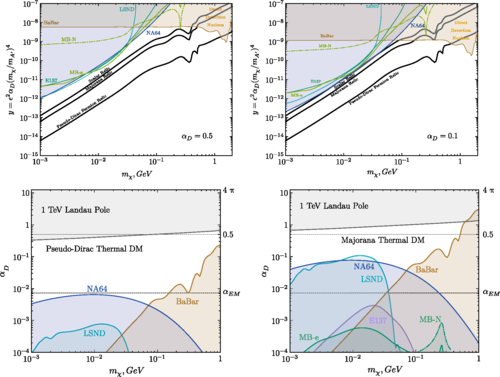
\includegraphics[scale=0.8]{\pdirfour/tldra-complete.png}
  \caption{The top rows show the NA64 limits in the $\dmyplane$ plane obtained for $\alpha_D = 0.5$ (left panel) and $\alpha_D = 0.1$ (right panel) from the full 2016-2018 data set. The bottom rows shows the same constraint in the $\dmaplane$ for the pseudo-Dirac (left panel) and Majorana (right panel) Dark matter. The limits are shown in comparison with the bounds obtained from the results of the LNSD \cite{deNiverville:2011it}, E137 \cite{e137}, MiniBooNE \cite{Aguilar-Arevalo:2018wea}, BABAR \cite{babar1} and direct detection experiments \cite{Essig:2012yx}. The favored parameters to account for the observed relic DM density for the scalar, pseudo-Dirac and Majorana type of light DM are shown as the lowest solid line in top plots \cite{Berlin:2018bsc}.}
  \label{fig:dm-alpha-excl}
\end{figure}
%%% Local Variables:
%%% mode: latex
%%% TeX-master: "../PhDthesis"
%%% End:
